\chapter{静磁场}

\section{静磁近似与 Maxwell 方程的退化}

静磁场讨论不随时间变化的电流分布所产生的磁场。在静态情形下，场量不显含时间，因而
\[
\frac{\partial \bm{E}}{\partial t}=0,
\qquad
\frac{\partial \bm{B}}{\partial t}=0.
\]
Maxwell 方程组化为
\begin{equation}
	\begin{dcases}
		\bm{\nabla}\cdot\bm{E}=\frac{\rho}{\varepsilon_{0}}, \\[6pt]
		\bm{\nabla}\times\bm{E}=\bm{0}, \\[6pt]
		\bm{\nabla}\cdot\bm{B}=0, \\[6pt]
		\bm{\nabla}\times\bm{B}=\mu_{0}\bm{j}.
	\end{dcases}
	\label{eq:maxwell-static}
\end{equation}
静态条件下电场方程和磁场方程相互分离。上一章讨论的是由静止电荷分布决定的静电场。本章讨论由稳恒电流分布决定的静磁场，其基本方程为
\begin{equation}
	\bm{\nabla}\cdot\bm{B}=0,
	\qquad
	\bm{\nabla}\times\bm{B}
	=
	\mu_{0}\bm{j}.
	\label{eq:11:magnetostatic-equations}
\end{equation}

第一式说明磁场没有散度源。磁感线没有起点和终点，只能闭合或延伸到无穷远。第二式说明稳恒电流是磁场的旋涡源。这个结构与静电场有本质差别：静电场由电荷作为散度源，而静磁场由电流作为旋度源。

静磁近似并不是简单地令电场为零。对于同时存在静止电荷和稳恒电流的体系，静电场和静磁场可以分别由各自的静态方程求得。本章的重点是磁场部分，即电流分布、磁矢势、磁场边界条件、磁矢势的多极展开、磁标势、磁介质和静磁能。

\section{稳恒电流与电流密度}

电流密度 $\bm{j}$ 描述单位面积上通过的电荷流率。若取有向面元 $\dif\bm{a}$，穿过该面元的电流为
\[
\dif I
=
\bm{j}\cdot\dif\bm{a}.
\]
穿过有限曲面 $S$ 的总电流为
\[
I
=
\int_{S}\bm{j}\cdot\dif\bm{a}.
\]

若一种电荷密度为 $\rho$ 的载流子以宏观平均速度 $\bm{v}$ 运动，则
\[
\bm{j}=\rho\bm{v}.
\]
若体系中存在多种载流子，电流密度应取各类载流子贡献之和：
\[
\bm{j}
=
\sum_{\alpha}
\rho_{\alpha}\bm{v}_{\alpha}.
\]
这里的速度是经过宏观平均后的漂移速度，而不是粒子热运动速度的简单大小。

电荷守恒由连续性方程表示：
\[
\frac{\partial\rho}{\partial t}
+
\bm{\nabla}\cdot\bm{j}=0.
\]
在静磁场中，电荷密度不随时间变化，即 $\partial\rho/\partial t=0$，于是
\begin{equation}
	\bm{\nabla}\cdot\bm{j}=0.
	\label{eq:11:steady-current-continuity}
\end{equation}
这说明稳恒电流线不能在空间中突然终止。它们必须闭合，或者延伸到无穷远。这个性质对于后面磁矢势远场展开非常重要。

电流可以用体电流、面电流或线电流描述。体电流密度为 $\bm{j}$，单位为 $\mathrm{A}/\mathrm{m}^{2}$。若电流限制在一个薄层中，可以用面电流密度 $\bm{K}$ 描述，单位为 $\mathrm{A}/\mathrm{m}$。若电流限制在细导线中，则用线电流 $I$ 描述。

设细导线的有向线元为 $\dif\bm{l}'$。在线电流近似下，体电流积分可替换为
\[
\int \bm{j}(\bm{r}')\,\dif^{3}r'
\quad \longrightarrow \quad
I\int \dif\bm{l}'.
\]
这种写法表示在导线横截面上已经完成了对体电流密度的积分。后面由体电流公式得到线电流公式时，将使用这一对应关系。

\section{磁矢势与规范自由}

静磁场满足
\[
\bm{\nabla}\cdot\bm{B}=0.
\]
散度为零的矢量场可以表示为另一个矢量场的旋度。因此引入磁矢势 $\bm{A}$：
\begin{equation}
	\bm{B}
	=
	\bm{\nabla}\times\bm{A}.
	\label{eq:11:b-curl-a}
\end{equation}
这样 $\bm{\nabla}\cdot\bm{B}=0$ 自动满足，因为任意旋度场的散度恒为零。

磁矢势并不唯一。若令
\[
\bm{A}'
=
\bm{A}
+
\bm{\nabla}\chi,
\]
其中 $\chi$ 是任意足够光滑的标量函数，则
\[
\bm{\nabla}\times\bm{A}'
=
\bm{\nabla}\times\bm{A}
+
\bm{\nabla}\times(\bm{\nabla}\chi)
=
\bm{\nabla}\times\bm{A}.
\]
因此 $\bm{A}$ 和 $\bm{A}'$ 给出同一个磁场。这种不唯一性称为规范自由。

在静磁场中，常用 Coulomb 规范：
\begin{equation}
	\bm{\nabla}\cdot\bm{A}=0.
	\label{eq:11:coulomb-gauge}
\end{equation}
该规范使磁矢势方程化为与静电势方程相似的 Poisson 方程。规范选择并不改变磁场本身，而是选择了描述同一磁场的一种方便的矢势代表。

含时电磁场中还常使用 Lorenz 规范
\[
\bm{\nabla}\cdot\bm{A}
+
\frac{1}{c^{2}}\frac{\partial\phi}{\partial t}
=0.
\]
它同时约束标量势和矢势，使二者满足解耦的波动方程。在本章的静态条件下，
$\partial\phi/\partial t=0$，Lorenz 规范退化为
$\bm{\nabla}\cdot\bm{A}=0$，与这里采用的 Coulomb 规范形式相同。因此本章无需另行建立一套 Lorenz 规范求解方法；其含时意义以及由此得到的推迟势将在下一章讨论。

\section{磁矢势的 Poisson 方程}

把
\[
\bm{B}
=
\bm{\nabla}\times\bm{A}
\]
代入静磁方程
\[
\bm{\nabla}\times\bm{B}
=
\mu_{0}\bm{j},
\]
得到
\[
\bm{\nabla}\times(\bm{\nabla}\times\bm{A})
=
\mu_{0}\bm{j}.
\]
利用恒等式
\[
\bm{\nabla}\times(\bm{\nabla}\times\bm{A})
=
\bm{\nabla}(\bm{\nabla}\cdot\bm{A})
-
\nabla^{2}\bm{A},
\]
并取 Coulomb 规范 \eqref{eq:11:coulomb-gauge}，得到
\begin{equation}
	\nabla^{2}\bm{A}
	=
	-\mu_{0}\bm{j}.
	\label{eq:11:vector-poisson-a}
\end{equation}
这是磁矢势的 Poisson 方程。它的三个分量分别满足
\[
\nabla^{2}A_{i}
=
-\mu_{0}j_{i}.
\]
这个方程与静电势方程
\[
\nabla^{2}\phi
=
-\frac{\rho}{\varepsilon_{0}}
\]
形式平行。静电场用标量势 $\phi$ 描述，静磁场用矢量势 $\bm{A}$ 描述。

在无界空间中，若电流分布局域，并取 $\bm{A}$ 在无穷远处趋于零，则 \eqref{eq:11:vector-poisson-a} 的解为
\begin{equation}
	\bm{A}(\bm{r})
	=
	\frac{\mu_{0}}{4\pi}
	\int
	\frac{\bm{j}(\bm{r}')}{|\bm{r}-\bm{r}'|}
	\,\dif^{3}r'.
	\label{eq:11:a-green-solution}
\end{equation}
这里 $\bm{r}'$ 是源点，$\bm{r}$ 是观察点。

这个解自动满足 Coulomb 规范。事实上，
\[
\bm{\nabla}\cdot\bm{A}(\bm{r})
=
\frac{\mu_{0}}{4\pi}
\int
\bm{j}(\bm{r}')\cdot
\bm{\nabla}
\frac{1}{|\bm{r}-\bm{r}'|}
\,\dif^{3}r'.
\]
由于
\[
\bm{\nabla}
\frac{1}{|\bm{r}-\bm{r}'|}
=
-\bm{\nabla}'
\frac{1}{|\bm{r}-\bm{r}'|},
\]
有
\[
\bm{\nabla}\cdot\bm{A}(\bm{r})
=
-\frac{\mu_{0}}{4\pi}
\int
\bm{j}(\bm{r}')\cdot
\bm{\nabla}'
\frac{1}{|\bm{r}-\bm{r}'|}
\,\dif^{3}r'.
\]
利用
\[
\bm{\nabla}'\cdot
\left(
\frac{\bm{j}(\bm{r}')}{|\bm{r}-\bm{r}'|}
\right)
=
\frac{\bm{\nabla}'\cdot\bm{j}(\bm{r}')}{|\bm{r}-\bm{r}'|}
+
\bm{j}(\bm{r}')\cdot
\bm{\nabla}'
\frac{1}{|\bm{r}-\bm{r}'|},
\]
并使用稳恒电流条件 $\bm{\nabla}'\cdot\bm{j}=0$，可知 $\bm{\nabla}\cdot\bm{A}$ 化为无穷远处的边界项。对于局域电流分布，该边界项为零。因此 \eqref{eq:11:a-green-solution} 与 Coulomb 规范相容。

\section{Biot--Savart 形式}

由磁矢势解 \eqref{eq:11:a-green-solution} 和 $\bm{B}=\bm{\nabla}\times\bm{A}$ 可得磁场积分形式。因为 $\bm{j}(\bm{r}')$ 与观察点坐标 $\bm{r}$ 无关，有
\[
\bm{\nabla}\times
\left(
\frac{\bm{j}(\bm{r}')}{|\bm{r}-\bm{r}'|}
\right)
=
\bm{\nabla}
\left(
\frac{1}{|\bm{r}-\bm{r}'|}
\right)
\times
\bm{j}(\bm{r}').
\]
又
\[
\bm{\nabla}
\left(
\frac{1}{|\bm{r}-\bm{r}'|}
\right)
=
-\frac{\bm{r}-\bm{r}'}{|\bm{r}-\bm{r}'|^{3}},
\]
因此
\[
\bm{\nabla}
\left(
\frac{1}{|\bm{r}-\bm{r}'|}
\right)
\times
\bm{j}(\bm{r}')
=
\frac{\bm{j}(\bm{r}')\times(\bm{r}-\bm{r}')}{|\bm{r}-\bm{r}'|^{3}}.
\]
于是得到
\begin{equation}
	\bm{B}(\bm{r})
	=
	\frac{\mu_{0}}{4\pi}
	\int
	\frac{
		\bm{j}(\bm{r}')\times(\bm{r}-\bm{r}')
	}{
		|\bm{r}-\bm{r}'|^{3}
	}
	\,\dif^{3}r'.
	\label{eq:11:biot-savart-volume}
\end{equation}
这就是静磁场的 Biot--Savart 形式。
\begin{figure}[h]
	\centering
	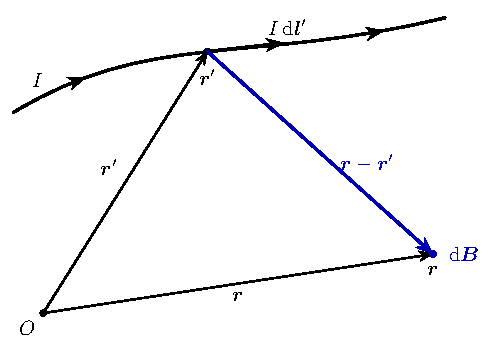
\includegraphics[width=0.4\linewidth]{figure/fig11.1}
	\caption[Biot--Savart定律]{Biot--Savart定律}
	\label{fig:11.1}
\end{figure}

对于细导线电流，使用
\[
\bm{j}(\bm{r}')\,\dif^{3}r'
\quad \longrightarrow \quad
I\,\dif\bm{l}',
\]
可得线电流形式
\begin{equation}
	\bm{B}(\bm{r})
	=
	\frac{\mu_{0}I}{4\pi}
	\int
	\frac{
		\dif\bm{l}'\times(\bm{r}-\bm{r}')
	}{
		|\bm{r}-\bm{r}'|^{3}
	}.
	\label{eq:11:biot-savart-line}
\end{equation}

作为例子，考虑无限长直导线，电流沿 $z$ 方向。由于柱面对称性，磁场只能沿方位角方向，且大小只依赖到导线的距离 $s$。由 \eqref{eq:11:biot-savart-line} 可直接得到
\[
\bm{B}(s)
=
\frac{\mu_{0}I}{2\pi s}\bm{e}_{\varphi}.
\]
这个结果也可以由下一节的 Ampere 环路定理更快得到。
\begin{figure}[h]
	\centering
	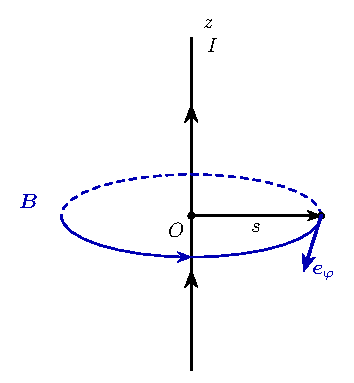
\includegraphics[width=0.3\linewidth]{figure/fig11.2}
	\caption[无限长直导线的磁场]{无限长直导线的磁场}
	\label{fig:11.2}
\end{figure}
\begin{example}{无限长直导线的磁场}{11,1}
	无限长直导线沿 $z$ 轴放置，电流为 $I$，方向沿 $+z$ 方向。求距离导线为 $s$ 处的磁场。
	
	\begin{solution}
		由于电流分布具有柱面对称性，磁场只能沿方位角方向。取观察点为
		$\bm{r}=s\bm{e}_{x}$，源点为
		$\bm{r}'=z'\bm{e}_{z}$，则
		\[
		\dif\bm{l}'=\dif z'\bm{e}_{z},
		\qquad
		\bm{r}-\bm{r}'
		=
		s\bm{e}_{x}-z'\bm{e}_{z}.
		\]
		因而
		\[
		\dif\bm{l}'\times(\bm{r}-\bm{r}')
		=
		s\,\dif z'\bm{e}_{y}.
		\]
		由 Biot--Savart 公式，
		\[
		\bm{B}(s)
		=
		\frac{\mu_{0}I}{4\pi}
		\int_{-\infty}^{\infty}
		\frac{s\,\dif z'}{(s^{2}+z'^{2})^{3/2}}
		\bm{e}_{y}.
		\]
		利用
		\[
		\int_{-\infty}^{\infty}
		\frac{s\,\dif z'}{(s^{2}+z'^{2})^{3/2}}
		=
		\frac{2}{s},
		\]
		得到
		\[
		\bm{B}(s)
		=
		\frac{\mu_{0}I}{2\pi s}\bm{e}_{y}.
		\]
		在任意方位角处，这一方向就是 $\bm{e}_{\varphi}$，故
		\[
		\bm{B}(s)
		=
		\frac{\mu_{0}I}{2\pi s}\bm{e}_{\varphi}.
		\]
		下一节将看到，利用 Ampere 环路定理可更直接地得到同一结果。
	\end{solution}
\end{example}


\section{Ampere 环路定理与高对称磁场}

静磁方程
\[
\bm{\nabla}\times\bm{B}
=
\mu_{0}\bm{j}
\]
在任意有向曲面 $S$ 上积分，得
\[
\int_{S}
(\bm{\nabla}\times\bm{B})\cdot\dif\bm{a}
=
\mu_{0}
\int_{S}
\bm{j}\cdot\dif\bm{a}.
\]
由 Stokes 定理，左边化为边界曲线 $C=\partial S$ 上的环量：
\[
\oint_{C}
\bm{B}\cdot\dif\bm{l}
=
\mu_{0}
\int_{S}
\bm{j}\cdot\dif\bm{a}.
\]
记穿过曲面 $S$ 的总电流为
\[
I_{\mathrm{enc}}
=
\int_{S}
\bm{j}\cdot\dif\bm{a},
\]
得到
\begin{equation}
	\oint_{C}
	\bm{B}\cdot\dif\bm{l}
	=
	\mu_{0}I_{\mathrm{enc}}.
	\label{eq:11:ampere-law}
\end{equation}
这就是静磁场的 Ampere 环路定理。

Ampere 环路定理在具有高度对称性的磁场中尤其有效。对无限长直导线，取以导线为轴、半径为 $s$ 的圆形回路。磁场沿切向，且在回路上大小相同，于是
\[
\oint_{C}\bm{B}\cdot\dif\bm{l}
=
B(s)2\pi s.
\]
回路所围电流为 $I$，因此
\[
B(s)2\pi s
=
\mu_{0}I,
\]
即
\[
\bm{B}(s)
=
\frac{\mu_{0}I}{2\pi s}\bm{e}_{\varphi}.
\]

对长直螺线管，设单位长度匝数为 $n$，每匝电流为 $I$。理想长螺线管内部磁场近似均匀并沿轴向，外部磁场可忽略。取穿过管内外的矩形回路，环路定理给出
\[
Bl
=
\mu_{0}nIl,
\]
从而
\[
B
=
\mu_{0}nI.
\]
这个结果描述的是远离端部的内部磁场。

对环形螺线管，设总匝数为 $N$，电流为 $I$。在环形芯内部取半径为 $s$ 的圆形回路，则
\[
B(s)2\pi s
=
\mu_{0}NI,
\]
所以
\[
B(s)
=
\frac{\mu_{0}NI}{2\pi s}.
\]

\begin{example}{长直螺线管内部磁场}{11,2}
	设长直螺线管单位长度匝数为 $n$，每匝电流为 $I$。忽略端部效应，求螺线管内部磁场。
	
	\begin{solution}
		理想长螺线管内部磁场近似均匀并沿轴向，外部磁场近似为零。取一个矩形 Ampere 回路，其中一条长边位于螺线管内部并沿轴向，长度为 $l$；另一条长边位于螺线管外部。
		
		回路积分中，内部长边给出
		\[
		\int_{\mathrm{in}}\bm{B}\cdot\dif\bm{l}=Bl.
		\]
		外部磁场近似为零，短边与磁场垂直，因此其余部分贡献为零。矩形回路所围的总电流为
		\[
		I_{\mathrm{enc}}=nlI.
		\]
		由 Ampere 环路定理，
		\[
		Bl=\mu_{0}nlI.
		\]
		因此螺线管内部磁场为
		\[
		\bm{B}
		=
		\mu_{0}nI\,\bm{e}_{z},
		\]
		方向由线圈电流方向按右手定则确定。
	\end{solution}
\end{example}

这些例子说明，Ampere 环路定理本质上是静磁方程的积分形式。它不是一般积分公式的替代品，而是在对称性足够高时给出直接求解磁场的简洁方法。

\section{磁场的边界条件}

磁场边界条件来自静磁方程的积分形式。设界面两侧区域分别为 $1$ 和 $2$，法向单位矢量 $\bm{n}$ 从区域 $1$ 指向区域 $2$。界面两侧磁场分别为 $\bm{B}_{1}$ 和 $\bm{B}_{2}$。

先考虑法向分量。取一个跨过界面的薄柱体作为 Gauss 面。由
\[
\bm{\nabla}\cdot\bm{B}=0
\]
可得
\[
\oint \bm{B}\cdot\dif\bm{a}=0.
\]
令柱体高度趋于零，侧面积贡献消失，只剩上下底面贡献：
\[
\bm{n}\cdot\bm{B}_{2}\Delta A
-
\bm{n}\cdot\bm{B}_{1}\Delta A=0.
\]
因此
\begin{equation}
	\bm{n}\cdot(\bm{B}_{2}-\bm{B}_{1})=0.
	\label{eq:11:boundary-normal-b}
\end{equation}
磁场法向分量连续。这是无磁单极条件在界面上的表现。

再考虑切向分量。取一个跨过界面的狭长矩形回路，长边平行于界面，短边垂直于界面。若界面上存在面电流密度 $\bm{K}$，由 Ampere 环路定理可得
\[
\oint \bm{B}\cdot\dif\bm{l}
=
\mu_{0}I_{\mathrm{enc}}.
\]
令短边长度趋于零，短边贡献消失。穿过矩形回路的电流为 $\bm{K}\cdot\bm{t}\Delta l$，其中 $\bm{t}$ 是与回路面法向相应的切向方向。整理后得到
\begin{equation}
	\bm{n}\times(\bm{B}_{2}-\bm{B}_{1})
	=
	\mu_{0}\bm{K}.
	\label{eq:11:boundary-tangential-b}
\end{equation}
若界面上没有面电流，则磁场切向分量也连续。

与静电边界条件相比，静磁边界条件呈现出对偶结构。静电场的法向分量因面电荷而跃变，切向分量连续；静磁场的法向分量连续，切向分量因面电流而跃变。

\begin{example}{无限大面电流的磁场跃变}{11,3}
	设 $z=0$ 平面上有均匀面电流密度
	\[
	\bm{K}=K\bm{e}_{x}.
	\]
	求平面两侧的磁场。
	
	\begin{solution}
		系统在 $x$ 与 $y$ 方向平移不变。由对称性，磁场只能位于平面内并垂直于电流方向，因此可设
		\[
		\bm{B}_{+}=B_{+}\bm{e}_{y},
		\qquad
		\bm{B}_{-}=B_{-}\bm{e}_{y},
		\]
		其中 $+$ 表示 $z>0$ 一侧，$-$ 表示 $z<0$ 一侧。
		
		面电流边界条件为
		\[
		\bm{n}\times(\bm{B}_{+}-\bm{B}_{-})
		=
		\mu_{0}\bm{K},
		\]
		这里 $\bm{n}=\bm{e}_{z}$。代入得
		\[
		\bm{e}_{z}\times[(B_{+}-B_{-})\bm{e}_{y}]
		=
		\mu_{0}K\bm{e}_{x}.
		\]
		由于 $\bm{e}_{z}\times\bm{e}_{y}=-\bm{e}_{x}$，所以
		\[
		-(B_{+}-B_{-})\bm{e}_{x}
		=
		\mu_{0}K\bm{e}_{x}.
		\]
		即
		\[
		B_{-}-B_{+}=\mu_{0}K.
		\]
		由上下对称性可知两侧磁场大小相等、方向相反，所以
		\[
		B_{-}=\frac{\mu_{0}K}{2},
		\qquad
		B_{+}=-\frac{\mu_{0}K}{2}.
		\]
		因此
		\[
		\bm{B}_{+}
		=
		-\frac{\mu_{0}K}{2}\bm{e}_{y},
		\qquad
		\bm{B}_{-}
		=
		\frac{\mu_{0}K}{2}\bm{e}_{y}.
		\]
	\end{solution}
\end{example}


\section{磁矢势的多极展开}

上一章中，静电势的远场结构可以由 Coulomb 核函数的展开得到。静磁场也有类似的远场分析，但展开对象不再是标量势 $\phi$，而是磁矢势 $\bm{A}$。对于局域稳恒电流分布，磁矢势的自由空间解为
\[
\bm{A}(\bm{r})
=
\frac{\mu_{0}}{4\pi}
\int
\frac{\bm{j}(\bm{r}')}{|\bm{r}-\bm{r}'|}
\,\dif^{3}r'.
\]
设电流分布局域在原点附近，观察点满足 $r\gg r'$。此时可以把核函数 $1/|\bm{r}-\bm{r}'|$ 按 $r'/r$ 展开。这样得到的展开称为磁矢势的多极展开。

与静电多极展开相比，静磁多极展开有一个重要差别。静电势的最低阶可以是电单极项，即总电荷项；而局域稳恒电流没有磁单极远场。静磁远场的最低阶通常是磁偶极项。

\subsection{远场展开的基本形式}

对远场点 $r\gg r'$，有
\[
\frac{1}{|\bm{r}-\bm{r}'|}
=
\frac{1}{r}
+
\frac{\bm{r}\cdot\bm{r}'}{r^{3}}
+\cdots.
\]
代入磁矢势积分式，得到
\[
\bm{A}(\bm{r})
=
\frac{\mu_{0}}{4\pi}
\left[
\frac{1}{r}
\int
\bm{j}(\bm{r}')
\,\dif^{3}r'
+
\frac{x_{k}}{r^{3}}
\int
x'_{k}
\bm{j}(\bm{r}')
\,\dif^{3}r'
+\cdots
\right].
\]
这里采用 Einstein 求和约定。第一项表面上与静电势的单极项类似，但对于局域稳恒电流，它实际上为零。

为了看清这一点，考察任意一个分量 $j_i$。由恒等式
\[
\bm{\nabla}'\cdot(x'_i\bm{j})
=
j_i
+
x'_i\bm{\nabla}'\cdot\bm{j}
\]
以及稳恒电流条件 $\bm{\nabla}'\cdot\bm{j}=0$，可得
\[
j_i
=
\bm{\nabla}'\cdot(x'_i\bm{j}).
\]
对整个空间积分，并假设电流分布局域，边界项在无穷远处消失，于是
\begin{equation}
	\int
	\bm{j}(\bm{r}')
	\,\dif^{3}r'
	=
	0.
	\label{eq:11:current-monopole-vanishes}
\end{equation}
因此，局域稳恒电流的磁矢势没有 $1/r$ 阶的电流单极项。

\subsection{稳恒电流约束与磁偶极矩}

磁矢势的最低阶非零项来自一阶矩。定义
\[
M_{ik}
=
\int
x'_{k}j_i(\bm{r}')
\,\dif^{3}r'.
\]
稳恒电流还给出 $M_{ik}$ 的对称部分为零。事实上，
\[
\bm{\nabla}'\cdot(x'_ix'_k\bm{j})
=
x'_k j_i
+
x'_i j_k
+
x'_ix'_k\bm{\nabla}'\cdot\bm{j}.
\]
由于 $\bm{\nabla}'\cdot\bm{j}=0$，对空间积分并令边界项消失，得到
\[
M_{ik}+M_{ki}=0.
\]
所以 $M_{ik}$ 是反对称张量。三维空间中的反对称二阶张量可以用一个轴矢量表示。定义磁偶极矩
\begin{equation}
	\bm{m}
	=
	\frac{1}{2}
	\int
	\bm{r}'\times\bm{j}(\bm{r}')
	\,\dif^{3}r'.
	\label{eq:11:magnetic-dipole-moment}
\end{equation}
用分量表示，即
\[
m_l
=
\frac{1}{2}
\varepsilon_{lki}M_{ik}.
\]
反过来，
\[
M_{ik}
=
\varepsilon_{kil}m_l.
\]
因此，磁矢势的一阶项为
\[
A_i(\bm{r})
=
\frac{\mu_{0}}{4\pi}
\frac{x_k}{r^{3}}
M_{ik}
=
\frac{\mu_{0}}{4\pi}
\frac{x_k}{r^{3}}
\varepsilon_{kil}m_l.
\]
这正是矢量 $\bm{m}\times\bm{r}$ 的第 $i$ 个分量，于是得到
\begin{equation}
	\bm{A}(\bm{r})
	=
	\frac{\mu_{0}}{4\pi}
	\frac{\bm{m}\times\bm{r}}{r^{3}}.
	\label{eq:11:magnetic-dipole-a}
\end{equation}
这就是局域稳恒电流分布远场磁矢势的主导项。

对于平面细线闭合电流回路，磁偶极矩可化为更直观的形式：
\[
\bm{m}
=
I\bm{S},
\]
其中 $\bm{S}$ 是由回路方向按右手定则确定的有向面积矢量。这个结果说明，磁偶极矩描述的是闭合电流与其所围面积共同决定的远场效应。

\subsection{磁偶极场}

由 $\bm{B}=\bm{\nabla}\times\bm{A}$ 可得磁偶极子的远场磁场。在源外区域 $r\neq 0$，
\begin{equation}
	\bm{B}(\bm{r})
	=
	\frac{\mu_{0}}{4\pi}
	\frac{
		3\hat{\bm{r}}(\bm{m}\cdot\hat{\bm{r}})
		-
		\bm{m}
	}{r^{3}}.
	\label{eq:11:magnetic-dipole-b}
\end{equation}
这个表达式与电偶极场具有相似的角分布，但物理来源不同。电偶极矩描述正负电荷中心的分离；磁偶极矩描述局域闭合电流的面积效应。由于 $\bm{\nabla}\cdot\bm{B}=0$，局域稳恒电流分布不存在磁单极远场，最低阶通常是磁偶极项。

\begin{example}{圆形电流环的磁偶极矩}{11,4}
	半径为 $a$ 的圆形导线位于 $xy$ 平面内，电流为 $I$，从 $+z$ 方向看为逆时针方向。求该电流环的磁偶极矩，并写出远场磁矢势的主导项。
	
	\begin{solution}
		平面闭合电流回路的磁偶极矩为
		\[
		\bm{m}=I\bm{S}.
		\]
		圆形回路的面积为
		\[
		S=\pi a^{2}.
		\]
		电流从 $+z$ 方向看为逆时针方向，由右手定则，有向面积矢量沿 $+z$ 方向，因此
		\[
		\bm{m}
		=
		I\pi a^{2}\bm{e}_{z}.
		\]
		远离电流环时，磁矢势的主导项为磁偶极项：
		\[
		\bm{A}(\bm{r})
		=
		\frac{\mu_{0}}{4\pi}
		\frac{\bm{m}\times\bm{r}}{r^{3}}.
		\]
		代入 $\bm{m}=I\pi a^{2}\bm{e}_{z}$，得
		\[
		\bm{A}(\bm{r})
		=
		\frac{\mu_{0}I\pi a^{2}}{4\pi}
		\frac{\bm{e}_{z}\times\bm{r}}{r^{3}}.
		\]
		在球坐标中，$\bm{e}_{z}\times\bm{r}=r\sin\theta\,\bm{e}_{\varphi}$，所以
		\[
		\bm{A}(\bm{r})
		=
		\frac{\mu_{0}Ia^{2}}{4}
		\frac{\sin\theta}{r^{2}}\bm{e}_{\varphi}.
		\]
		该式是圆形电流环在远场区域的磁矢势主导项。
	\end{solution}
\end{example}

\section{磁标势与静磁场的边值问题}

磁矢势是静磁场的一般势函数描述。只要
\[
\bm{\nabla}\cdot\bm{B}=0,
\]
就可以在适当条件下写
\[
\bm{B}
=
\bm{\nabla}\times\bm{A}.
\]
因此，在有电流区域中，磁矢势是更基本的工具。

磁标势的适用范围更窄。若某一区域中没有电流，
\[
\bm{j}=0,
\]
则静磁方程给出
\[
\bm{\nabla}\times\bm{B}=0.
\]
如果该无电流区域还是单连通的，就可以引入磁标势 $\Phi_{\mathrm{m}}$，使
\begin{equation}
	\bm{B}
	=
	-\mu_{0}\bm{\nabla}\Phi_{\mathrm{m}}.
	\label{eq:11:magnetic-scalar-potential-vacuum}
\end{equation}
再由
\[
\bm{\nabla}\cdot\bm{B}=0
\]
得到
\begin{equation}
	\nabla^{2}\Phi_{\mathrm{m}}=0.
	\label{eq:11:magnetic-scalar-laplace}
\end{equation}
因此，在无电流单连通区域中，磁标势满足 Laplace 方程。

这与静电势有形式上的类比，但不能把二者完全等同。静电场在静态条件下全局无旋，因此可以在没有拓扑障碍时用电势描述；静磁场只在无电流区域中无旋。若所讨论区域中存在电流，或者区域虽然局部无电流但环绕了外部电流，磁标势就不能作为单值全局势函数使用。

磁标势的边值问题由 Laplace 方程和磁场边界条件共同决定。若界面两侧没有面电流，则
\[
\bm{n}\times(\bm{B}_{2}-\bm{B}_{1})=0.
\]
在真空中，由 $\bm{B}=-\mu_{0}\bm{\nabla}\Phi_{\mathrm{m}}$ 可知，这通常对应磁标势在界面上的连续性。又由于
\[
\bm{n}\cdot(\bm{B}_{2}-\bm{B}_{1})=0,
\]
法向导数也要满足相应连续条件。若存在面电流，磁场切向分量发生跃变，磁标势描述就必须按区域分片处理。

在源外无电流区域，磁标势可按球谐函数展开。若源局域在原点附近，外部区域满足 Laplace 方程，则
\begin{equation}
	\Phi_{\mathrm{m}}(\bm{r})
	=
	\sum_{l=0}^{\infty}
	\sum_{m=-l}^{l}
	\frac{a_{lm}}{r^{l+1}}
	Y_{lm}(\theta,\varphi).
	\label{eq:11:magnetic-scalar-spherical-expansion}
\end{equation}
由于不存在磁单极，局域稳恒电流的外部磁标势没有物理磁单极项。最低阶通常是磁偶极项。

由磁偶极场 \eqref{eq:11:magnetic-dipole-b} 可反推出源外磁标势：
\begin{equation}
	\Phi_{\mathrm{m}}(\bm{r})
	=
	\frac{1}{4\pi}
	\frac{\bm{m}\cdot\hat{\bm{r}}}{r^{2}}
	=
	\frac{1}{4\pi}
	\frac{\bm{m}\cdot\bm{r}}{r^{3}}.
	\label{eq:11:magnetic-dipole-scalar-potential}
\end{equation}
直接计算可得
\[
-\mu_{0}\bm{\nabla}\Phi_{\mathrm{m}}
=
\frac{\mu_{0}}{4\pi}
\frac{
	3\hat{\bm{r}}(\bm{m}\cdot\hat{\bm{r}})
	-
	\bm{m}
}{r^{3}},
\]
与 \eqref{eq:11:magnetic-dipole-b} 一致。

\begin{example}{磁偶极子的磁标势}{11,5}
	设局域电流分布的磁偶极矩为 $\bm{m}=m\bm{e}_{z}$。在源外无电流区域，求它的磁标势和磁场。
	
	\begin{solution}
		源外无电流区域可用磁标势描述。磁偶极标势为
		\[
		\Phi_{\mathrm{m}}(\bm{r})
		=
		\frac{1}{4\pi}
		\frac{\bm{m}\cdot\hat{\bm{r}}}{r^{2}}.
		\]
		当 $\bm{m}=m\bm{e}_{z}$ 时，
		\[
		\bm{m}\cdot\hat{\bm{r}}
		=
		m\cos\theta,
		\]
		因此
		\[
		\Phi_{\mathrm{m}}(r,\theta)
		=
		\frac{m\cos\theta}{4\pi r^{2}}.
		\]
		在球坐标中，
		\[
		\bm{\nabla}\Phi_{\mathrm{m}}
		=
		\frac{\partial\Phi_{\mathrm{m}}}{\partial r}\bm{e}_{r}
		+
		\frac{1}{r}
		\frac{\partial\Phi_{\mathrm{m}}}{\partial\theta}\bm{e}_{\theta}.
		\]
		计算得
		\[
		\frac{\partial\Phi_{\mathrm{m}}}{\partial r}
		=
		-\frac{2m\cos\theta}{4\pi r^{3}},
		\qquad
		\frac{1}{r}
		\frac{\partial\Phi_{\mathrm{m}}}{\partial\theta}
		=
		-\frac{m\sin\theta}{4\pi r^{3}}.
		\]
		由 $\bm{B}=-\mu_{0}\bm{\nabla}\Phi_{\mathrm{m}}$，得到
		\[
		\bm{B}
		=
		\frac{\mu_{0}m}{4\pi r^{3}}
		\left(
		2\cos\theta\,\bm{e}_{r}
		+
		\sin\theta\,\bm{e}_{\theta}
		\right).
		\]
		这与磁偶极场
		\[
		\bm{B}
		=
		\frac{\mu_{0}}{4\pi}
		\frac{
			3\hat{\bm{r}}(\bm{m}\cdot\hat{\bm{r}})
			-
			\bm{m}
		}{r^{3}}
		\]
		完全一致。
	\end{solution}
\end{example}

磁标势的意义主要在于把真空中的无电流区域转化为 Laplace 方程的边值问题。它适合处理局域电流源的外部区域以及具有轴对称边界的外部磁场问题。但在包含电流的区域中，磁矢势仍然是更一般的描述。磁介质中以 $\bm{H}$ 定义的磁标势与这里的真空磁标势形式相近，但其源项和边界条件需要结合磁化强度重新推导，后文将对此作专门说明。

\section{磁场对电流分布的作用}

带电粒子在磁场中受到 Lorentz 力。对于给定的连续电流分布，若只讨论外部磁场对它的机械作用，磁力密度为
\begin{equation}
	\bm{f}_{\mathrm{m}}
	=
	\bm{j}\times\bm{B}_{\mathrm{ext}}.
	\label{eq:11:magnetic-force-density}
\end{equation}
区域 $V$ 内电流分布受到的总磁力为
\[
\bm{F}
=
\int_{V}
\bm{j}\times\bm{B}_{\mathrm{ext}}
\,\dif^{3}x.
\]
这里显式写出下标 $\mathrm{ext}$，是为了避免把理想线电流自身产生的奇异自场直接代入力公式。若研究有限尺度电流分布内部各部分之间的作用，则必须连同应力、形变和场动量一起处理，不能把总场简单地当作外场使用。

对细导线，体积分可化为线积分。若导线中电流为 $I$，线元为 $\dif\bm{l}$，则
\begin{equation}
	\dif\bm{F}
	=
	I\,\dif\bm{l}\times\bm{B}_{\mathrm{ext}}.
	\label{eq:11:line-current-force}
\end{equation}
有限导线段受到的力为
\[
\bm{F}
=
I\int
\dif\bm{l}\times\bm{B}_{\mathrm{ext}}.
\]

磁偶极矩在外磁场中受到力矩。设小电流回路位于近似均匀的外磁场中，其磁偶极矩为 $\bm{m}$。回路所受力矩为
\begin{equation}
	\bm{\tau}
	=
	\bm{m}\times\bm{B}_{\mathrm{ext}}.
	\label{eq:11:magnetic-dipole-torque}
\end{equation}
相应势能为
\begin{equation}
	U
	=
	-\bm{m}\cdot\bm{B}_{\mathrm{ext}}.
	\label{eq:11:magnetic-dipole-energy}
\end{equation}
若外磁场不均匀，并且磁偶极矩在空间变化尺度内可近似为常量，则磁偶极子受到的力可写为
\[
\bm{F}
=
\bm{\nabla}(\bm{m}\cdot\bm{B}_{\mathrm{ext}}).
\]
这些公式描述了电流回路与外磁场之间的机械作用。

\begin{example}{两根平行长直导线间的作用力}{11,6}
	两根无限长平行直导线相距 $d$，电流分别为 $I_{1}$ 和 $I_{2}$，方向相同。求单位长度导线之间的磁力。
	
	\begin{solution}
		第一根导线在第二根导线所在位置产生的磁场大小为
		\[
		B_{1}
		=
		\frac{\mu_{0}I_{1}}{2\pi d}.
		\]
		第二根导线中长度为 $l$ 的一段受到的磁力为
		\[
		\bm{F}_{2}
		=
		I_{2}\int \dif\bm{l}\times\bm{B}_{1}.
		\]
		由于 $\dif\bm{l}$ 与 $\bm{B}_{1}$ 垂直，且磁场在该导线处大小不随 $z$ 变化，磁力大小为
		\[
		F_{2}
		=
		I_{2}lB_{1}
		=
		I_{2}l\frac{\mu_{0}I_{1}}{2\pi d}.
		\]
		所以单位长度受力大小为
		\[
		\frac{F_{2}}{l}
		=
		\frac{\mu_{0}I_{1}I_{2}}{2\pi d}.
		\]
		方向由 $\dif\bm{l}\times\bm{B}$ 决定。若两电流同向，两导线相互吸引；若两电流反向，则相互排斥。
	\end{solution}
\end{example}


\section{磁介质中的静磁场}

物质中的磁性来自微观电流和微观磁偶极矩。宏观电磁学中，用磁化强度 $\bm{M}$ 描述介质内单位体积的磁偶极矩。介质中的总电流可以分为自由电流和束缚电流：
\[
\bm{j}
=
\bm{j}_{\mathrm{f}}
+
\bm{j}_{\mathrm{b}}.
\]
磁化强度对应的束缚体电流密度为
\begin{equation}
	\bm{j}_{\mathrm{b}}
	=
	\bm{\nabla}\times\bm{M}.
	\label{eq:11:bound-current-volume}
\end{equation}
在介质边界上，还存在束缚面电流密度
\begin{equation}
	\bm{K}_{\mathrm{b}}
	=
	\bm{M}\times\bm{n}.
	\label{eq:11:bound-current-surface}
\end{equation}
其中 $\bm{n}$ 是介质表面向外的法向单位矢量。

将总电流分解代入静磁方程：
\[
\bm{\nabla}\times\bm{B}
=
\mu_{0}
(\bm{j}_{\mathrm{f}}+\bm{j}_{\mathrm{b}}).
\]
再使用 \eqref{eq:11:bound-current-volume}，得
\[
\bm{\nabla}\times\bm{B}
=
\mu_{0}
(\bm{j}_{\mathrm{f}}+\bm{\nabla}\times\bm{M}).
\]
整理为
\[
\bm{\nabla}\times
\left(
\frac{\bm{B}}{\mu_{0}}-\bm{M}
\right)
=
\bm{j}_{\mathrm{f}}.
\]
因此定义磁场强度
\begin{equation}
	\bm{H}
	=
	\frac{\bm{B}}{\mu_{0}}
	-
	\bm{M}.
	\label{eq:11:h-definition}
\end{equation}
于是介质中的静磁方程写为
\begin{equation}
	\bm{\nabla}\times\bm{H}
	=
	\bm{j}_{\mathrm{f}},
	\qquad
	\bm{\nabla}\cdot\bm{B}=0.
	\label{eq:11:magnetostatics-in-matter}
\end{equation}

需要注意的是，$\bm{B}$ 和 $\bm{H}$ 的物理角色不同。进入 Lorentz 力的是 $\bm{B}$；$\bm{H}$ 是为了把自由电流和束缚电流分开处理而引入的辅助场。它的环量只由自由电流决定。

对线性各向同性介质，磁化强度与 $\bm{H}$ 成正比：
\[
\bm{M}
=
\chi_{\mathrm{m}}\bm{H},
\]
其中 $\chi_{\mathrm{m}}$ 是磁化率。由 \eqref{eq:11:h-definition} 得
\[
\bm{B}
=
\mu_{0}(\bm{H}+\bm{M})
=
\mu_{0}(1+\chi_{\mathrm{m}})\bm{H}.
\]
记
\[
\mu
=
\mu_{0}\mu_{\mathrm{r}}
=
\mu_{0}(1+\chi_{\mathrm{m}}),
\]
则
\begin{equation}
	\bm{B}
	=
	\mu\bm{H}.
	\label{eq:11:linear-magnetic-medium}
\end{equation}

磁介质的边界条件由 \eqref{eq:11:magnetostatics-in-matter} 给出。磁感应强度的法向分量满足
\[
\bm{n}\cdot(\bm{B}_{2}-\bm{B}_{1})=0.
\]
磁场强度的切向分量满足
\[
\bm{n}\times(\bm{H}_{2}-\bm{H}_{1})
=
\bm{K}_{\mathrm{f}},
\]
其中 $\bm{K}_{\mathrm{f}}$ 是界面上的自由面电流密度。若界面上没有自由面电流，则 $\bm{H}$ 的切向分量连续。

在不含自由电流的单连通区域中，
\[
\bm{\nabla}\times\bm{H}=0,
\]
因而可以定义磁介质中的磁标势
\begin{equation}
	\bm{H}
	=
	-\bm{\nabla}\Phi_{\mathrm{m}}.
	\label{eq:11:h-scalar-potential}
\end{equation}
将
\[
\bm{B}
=
\mu_{0}(\bm{H}+\bm{M})
\]
代入 $\bm{\nabla}\cdot\bm{B}=0$，得到
\begin{equation}
	\nabla^{2}\Phi_{\mathrm{m}}
	=
	\bm{\nabla}\cdot\bm{M}.
	\label{eq:11:magnetic-scalar-poisson-matter}
\end{equation}
因此，磁介质中的磁标势一般满足 Poisson 方程，而不一定满足 Laplace 方程。只有在磁化强度散度为零的均匀区域内，它才满足 Laplace 方程。

如果把
\[
\rho_{\mathrm{m}}
=
-\bm{\nabla}\cdot\bm{M},
\qquad
\sigma_{\mathrm{m}}
=
\bm{M}\cdot\bm{n}
\]
分别称为等效体磁荷密度和等效面磁荷密度，那么
\eqref{eq:11:magnetic-scalar-poisson-matter} 可以像静电 Poisson 方程一样求解。这里的磁荷只是描述磁化强度散度和边界效应的数学工具，并不表示存在基本磁单极。

设法向单位矢量 $\bm{n}$ 从介质 $1$ 指向介质 $2$，且界面上没有自由面电流。由 $\bm{H}$ 的切向分量连续，可取
\[
\Phi_{\mathrm{m},2}
=
\Phi_{\mathrm{m},1}
\]
作为势函数的连续条件。再由 $\bm{B}$ 的法向分量连续，得到
\begin{equation}
	\frac{\partial\Phi_{\mathrm{m},2}}{\partial n}
	-
	\frac{\partial\Phi_{\mathrm{m},1}}{\partial n}
	=
	\bm{n}\cdot(\bm{M}_{2}-\bm{M}_{1}).
	\label{eq:11:magnetic-scalar-boundary-matter}
\end{equation}
这组条件与真空磁标势的边界条件不同，差别正是由界面两侧磁化强度的跃变造成的。

\begin{example}{均匀磁化球体的内外磁场}{11,7}
	半径为 $R$ 的球体具有均匀磁化强度
	\[
	\bm{M}=M\bm{e}_{z}.
	\]
	球内外均无自由电流，球外为真空。求球内外的 $\bm{H}$ 和 $\bm{B}$。

	\begin{solution}
		球内 $\bm{\nabla}\cdot\bm{M}=0$，球外 $\bm{M}=0$，所以两个区域的磁标势都满足 Laplace 方程。体系关于 $z$ 轴对称，且边界数据正比于
		\[
		\bm{M}\cdot\bm{e}_{r}
		=
		M\cos\theta.
		\]
		因此只需要保留 $l=1$ 的轴对称解。要求球心处有限、无穷远处趋于零，可设
		\[
		\Phi_{\mathrm{in}}
		=
		a r\cos\theta,
		\qquad
		\Phi_{\mathrm{out}}
		=
		\frac{b\cos\theta}{r^{2}}.
		\]
		界面上没有自由面电流，磁标势连续，故
		\[
		aR
		=
		\frac{b}{R^{2}},
		\qquad
		b=aR^{3}.
		\]

		取法向从球内指向球外。此时
		$\bm{M}_{1}=M\bm{e}_{z}$、$\bm{M}_{2}=0$，由
		\eqref{eq:11:magnetic-scalar-boundary-matter}，
		\[
		\left.
		\frac{\partial\Phi_{\mathrm{out}}}{\partial r}
		\right|_{r=R}
		-
		\left.
		\frac{\partial\Phi_{\mathrm{in}}}{\partial r}
		\right|_{r=R}
		=
		-M\cos\theta.
		\]
		代入势函数并使用 $b=aR^{3}$，得到
		\[
		-2a\cos\theta-a\cos\theta
		=
		-M\cos\theta,
		\]
		所以
		\[
		a=\frac{M}{3},
		\qquad
		b=\frac{MR^{3}}{3}.
		\]

		球内磁标势为
		\[
		\Phi_{\mathrm{in}}
		=
		\frac{M}{3}r\cos\theta
		=
		\frac{M}{3}z.
		\]
		由 $\bm{H}=-\bm{\nabla}\Phi_{\mathrm{m}}$，
		\[
		\bm{H}_{\mathrm{in}}
		=
		-\frac{1}{3}\bm{M}.
		\]
		这个与磁化方向相反的均匀场称为退磁场，球体的退磁因子为 $1/3$。球内磁感应强度为
		\[
		\bm{B}_{\mathrm{in}}
		=
		\mu_{0}
		(\bm{H}_{\mathrm{in}}+\bm{M})
		=
		\frac{2}{3}\mu_{0}\bm{M}.
		\]

		球外磁标势为
		\[
		\Phi_{\mathrm{out}}
		=
		\frac{MR^{3}\cos\theta}{3r^{2}}.
		\]
		球体的总磁偶极矩为
		\[
		\bm{m}
		=
		\int_{V}\bm{M}\,\dif^{3}x
		=
		\frac{4\pi R^{3}}{3}\bm{M}.
		\]
		于是
		\[
		\Phi_{\mathrm{out}}
		=
		\frac{1}{4\pi}
		\frac{\bm{m}\cdot\hat{\bm{r}}}{r^{2}},
		\]
		说明球外磁场与位于球心、磁偶极矩为 $\bm{m}$ 的点磁偶极子完全相同：
		\[
		\bm{H}_{\mathrm{out}}
		=
		\frac{1}{4\pi r^{3}}
		\left[
		3\hat{\bm{r}}
		(\bm{m}\cdot\hat{\bm{r}})
		-
		\bm{m}
		\right],
		\qquad
		\bm{B}_{\mathrm{out}}
		=
		\mu_{0}\bm{H}_{\mathrm{out}}.
		\]
	\end{solution}
\end{example}

\section{静磁能、电感与互感}

静磁场具有能量。在真空中，磁场能量密度为
\[
u_{\mathrm{m}}
=
\frac{1}{2\mu_{0}}B^{2}.
\]
因此总磁能为
\begin{equation}
	U_{\mathrm{m}}
	=
	\frac{1}{2\mu_{0}}
	\int
	B^{2}\,\dif^{3}x.
	\label{eq:11:magnetic-energy-field}
\end{equation}

磁能也可以写成电流与磁矢势的形式：
\begin{equation}
	U_{\mathrm{m}}
	=
	\frac{1}{2}
	\int
	\bm{j}\cdot\bm{A}
	\,\dif^{3}x.
	\label{eq:11:magnetic-energy-current-a}
\end{equation}
下面说明它与 \eqref{eq:11:magnetic-energy-field} 的一致性。在真空中，
\[
\bm{j}
=
\frac{1}{\mu_{0}}\bm{\nabla}\times\bm{B}.
\]
代入 \eqref{eq:11:magnetic-energy-current-a}，得
\[
U_{\mathrm{m}}
=
\frac{1}{2\mu_{0}}
\int
\bm{A}\cdot(\bm{\nabla}\times\bm{B})
\,\dif^{3}x.
\]
使用恒等式
\[
\bm{\nabla}\cdot(\bm{B}\times\bm{A})
=
\bm{A}\cdot(\bm{\nabla}\times\bm{B})
-
\bm{B}\cdot(\bm{\nabla}\times\bm{A}),
\]
并取边界在无穷远处使表面积分消失，可得
\[
U_{\mathrm{m}}
=
\frac{1}{2\mu_{0}}
\int
\bm{B}\cdot(\bm{\nabla}\times\bm{A})
\,\dif^{3}x.
\]
由于 $\bm{\nabla}\times\bm{A}=\bm{B}$，于是
\[
U_{\mathrm{m}}
=
\frac{1}{2\mu_{0}}
\int
B^{2}\,\dif^{3}x.
\]

对于由若干细导线回路组成的系统，\eqref{eq:11:magnetic-energy-current-a} 可写成
\[
U_{\mathrm{m}}
=
\frac{1}{2}
\sum_{i}
I_{i}\Psi_{i},
\]
其中 $\Psi_{i}$ 是第 $i$ 个回路的磁链。若线圈有 $N_i$ 匝，并且每匝所穿磁通量都近似为 $\Phi_i$，则
\[
\Psi_i=N_i\Phi_i.
\]
对于单匝回路，磁链与磁通量相同。在线性系统中，磁链与各回路电流线性相关：
\[
\Psi_{i}
=
\sum_{j}L_{ij}I_{j}.
\]
于是
\[
U_{\mathrm{m}}
=
\frac{1}{2}
\sum_{i,j}
L_{ij}I_{i}I_{j}.
\]
对单个线圈，
\[
\Psi=LI,
\]
因而
\begin{equation}
	U_{\mathrm{m}}
	=
	\frac{1}{2}LI^{2}.
	\label{eq:11:self-inductance-energy}
\end{equation}
对两个回路，
\[
U_{\mathrm{m}}
=
\frac{1}{2}L_{1}I_{1}^{2}
+
\frac{1}{2}L_{2}I_{2}^{2}
+
MI_{1}I_{2},
\]
其中 $M=L_{12}=L_{21}$ 是互感，符号由两个回路磁通方向的取向约定决定。

对于两个彼此分离的细导线闭合回路，互感还可以直接由几何形状表示。由回路 $1$ 中的电流 $I_1$ 产生的磁矢势为
\[
\bm{A}_{1}(\bm{r}_{2})
=
\frac{\mu_{0}I_{1}}{4\pi}
\oint_{C_{1}}
\frac{\dif\bm{l}_{1}}{|\bm{r}_{2}-\bm{r}_{1}|}.
\]
回路 $2$ 中的磁通量可写为
\[
\Phi_{21}
=
\oint_{C_{2}}
\bm{A}_{1}\cdot\dif\bm{l}_{2}
=
M_{21}I_{1}.
\]
因此得到 Neumann 公式
\begin{equation}
	M_{21}
	=
	\frac{\mu_{0}}{4\pi}
	\oint_{C_{1}}
	\oint_{C_{2}}
	\frac{
		\dif\bm{l}_{1}\cdot\dif\bm{l}_{2}
	}{
		|\bm{r}_{2}-\bm{r}_{1}|
	}.
	\label{eq:11:neumann-mutual-inductance}
\end{equation}
交换两个回路只相当于交换积分次序，所以
\[
M_{12}=M_{21}.
\]
这给出了互感互易关系的直接证明。需要注意，不能简单地令两个理想细线回路重合来计算自感，因为当两个线元趋于同一点时积分核会发散。实际导线具有有限截面，其内部磁场和电流分布共同决定有限的自感。

对一般可逆磁化过程，磁场能量密度的增量满足
\begin{equation}
	\dif u_{\mathrm{m}}
	=
	\bm{H}\cdot\dif\bm{B}.
	\label{eq:11:magnetic-energy-increment}
\end{equation}
若介质为线性并且本构关系可逆，则从零场积分得到
\[
u_{\mathrm{m}}
=
\frac{1}{2}\bm{B}\cdot\bm{H}.
\]
总能量为
\[
U_{\mathrm{m}}
=
\frac{1}{2}
\int
\bm{B}\cdot\bm{H}
\,\dif^{3}x.
\]
若介质为线性各向同性，$\bm{B}=\mu\bm{H}$，则
\[
U_{\mathrm{m}}
=
\frac{1}{2}
\int
\mu H^{2}
\,\dif^{3}x
=
\frac{1}{2}
\int
\frac{B^{2}}{\mu}
\,\dif^{3}x.
\]
对于非线性介质，应沿实际磁化路径对
$\bm{H}\cdot\dif\bm{B}$ 积分，不能直接使用
$\bm{B}\cdot\bm{H}/2$。存在磁滞时，能量还与磁化历史有关，一个循环中的回线面积对应不可逆损耗。

\begin{example}{长直螺线管的自感系数}{11,8}
	长直螺线管长度为 $l$，截面积为 $S$，单位长度匝数为 $n$，总匝数为 $N=nl$。忽略端部效应，求其自感系数。
	
	\begin{solution}
		长直螺线管内部磁场为
		\[
		B=\mu_{0}nI.
		\]
		穿过每一匝的磁通量为
		\[
		\Phi_{1}=BS=\mu_{0}nIS.
		\]
		总磁链为
		\[
		\Psi=N\Phi_{1}
		=
		nl\,\mu_{0}nIS
		=
		\mu_{0}n^{2}lSI.
		\]
		自感系数定义为磁链与电流之比：
		\[
		L=\frac{\Psi}{I}.
		\]
		因此
		\[
		L
		=
		\mu_{0}n^{2}lS.
		\]
		也可以从磁能验证。螺线管内部磁能为
		\[
		U_{\mathrm{m}}
		=
		\frac{1}{2\mu_{0}}B^{2}lS
		=
		\frac{1}{2\mu_{0}}(\mu_{0}nI)^{2}lS
		=
		\frac{1}{2}\mu_{0}n^{2}lSI^{2}.
		\]
		与
		\[
		U_{\mathrm{m}}=\frac{1}{2}LI^{2}
		\]
		比较，同样得到
		\[
		L=\mu_{0}n^{2}lS.
		\]
	\end{solution}
\end{example}


\section{本章小结}

本章讨论了静磁场的基本理论。静磁场的基本方程为
\[
\bm{\nabla}\cdot\bm{B}=0,
\qquad
\bm{\nabla}\times\bm{B}
=
\mu_{0}\bm{j}.
\]
稳恒电流满足
\[
\bm{\nabla}\cdot\bm{j}=0.
\]
磁场没有散度源，因此可引入磁矢势
\[
\bm{B}
=
\bm{\nabla}\times\bm{A}.
\]
在 Coulomb 规范
\[
\bm{\nabla}\cdot\bm{A}=0
\]
下，磁矢势满足 Poisson 方程
\[
\nabla^{2}\bm{A}
=
-\mu_{0}\bm{j}.
\]
含时电磁场中的 Lorenz 规范在严格静态条件下退化为同一形式；它与 Coulomb 规范的实质区别只有在含时问题中才出现。
其无界空间解为
\[
\bm{A}(\bm{r})
=
\frac{\mu_{0}}{4\pi}
\int
\frac{\bm{j}(\bm{r}')}{|\bm{r}-\bm{r}'|}
\,\dif^{3}r'.
\]
取旋度得到磁场的 Biot--Savart 形式：
\[
\bm{B}(\bm{r})
=
\frac{\mu_{0}}{4\pi}
\int
\frac{
	\bm{j}(\bm{r}')\times(\bm{r}-\bm{r}')
}{
	|\bm{r}-\bm{r}'|^{3}
}
\,\dif^{3}r'.
\]

Ampere 环路定理为
\[
\oint_{C}\bm{B}\cdot\dif\bm{l}
=
\mu_{0}I_{\mathrm{enc}}.
\]
磁场边界条件为
\[
\bm{n}\cdot(\bm{B}_{2}-\bm{B}_{1})=0,
\qquad
\bm{n}\times(\bm{B}_{2}-\bm{B}_{1})
=
\mu_{0}\bm{K}.
\]

磁矢势的远场展开与静电势多极展开形式相似，但其物理结构不同。局域稳恒电流满足
\[
\int
\bm{j}(\bm{r}')
\,\dif^{3}r'
=
0,
\]
因此没有电流单极项。最低阶通常是磁偶极项。磁偶极矩为
\[
\bm{m}
=
\frac{1}{2}
\int
\bm{r}'\times\bm{j}(\bm{r}')
\,\dif^{3}r',
\]
远场磁矢势和磁场分别为
\[
\bm{A}(\bm{r})
=
\frac{\mu_{0}}{4\pi}
\frac{\bm{m}\times\bm{r}}{r^{3}},
\]
\[
\bm{B}(\bm{r})
=
\frac{\mu_{0}}{4\pi}
\frac{
	3\hat{\bm{r}}(\bm{m}\cdot\hat{\bm{r}})
	-
	\bm{m}
}{r^{3}}.
\]

在真空中的无电流单连通区域，可以引入磁标势
\[
\bm{B}
=
-\mu_{0}\bm{\nabla}\Phi_{\mathrm{m}},
\qquad
\nabla^{2}\Phi_{\mathrm{m}}=0.
\]
磁标势满足 Laplace 方程，因此可以像静电边值问题那样用分离变量和球谐展开处理。对于磁偶极远场，源外磁标势为
\[
\Phi_{\mathrm{m}}(\bm{r})
=
\frac{1}{4\pi}
\frac{\bm{m}\cdot\hat{\bm{r}}}{r^{2}}.
\]
但磁标势只适用于无电流单连通区域，不像静电势那样是静磁场的普遍势函数。

磁介质中引入磁化强度 $\bm{M}$，束缚电流满足
\[
\bm{j}_{\mathrm{b}}
=
\bm{\nabla}\times\bm{M},
\qquad
\bm{K}_{\mathrm{b}}
=
\bm{M}\times\bm{n}.
\]
定义
\[
\bm{H}
=
\frac{\bm{B}}{\mu_{0}}
-
\bm{M},
\]
则介质中的静磁方程为
\[
\bm{\nabla}\times\bm{H}
=
\bm{j}_{\mathrm{f}},
\qquad
\bm{\nabla}\cdot\bm{B}=0.
\]
在无自由电流的单连通磁介质区域中，可以改由
\[
\bm{H}
=
-\bm{\nabla}\Phi_{\mathrm{m}}
\]
定义磁标势，并得到
\[
\nabla^{2}\Phi_{\mathrm{m}}
=
\bm{\nabla}\cdot\bm{M}.
\]
均匀磁化球体内部的退磁场为
\[
\bm{H}_{\mathrm{in}}
=
-\frac{1}{3}\bm{M}.
\]

真空中的静磁能为
\[
U_{\mathrm{m}}
=
\frac{1}{2\mu_{0}}
\int
B^{2}\,\dif^{3}x
=
\frac{1}{2}
\int
\bm{j}\cdot\bm{A}\,\dif^{3}x.
\]
对单个线性回路，有
\[
U_{\mathrm{m}}
=
\frac{1}{2}LI^{2}.
\]
对多匝线圈，应使用磁链 $\Psi=N\Phi$ 定义自感。两个分离闭合回路的互感可由 Neumann 公式计算，并满足
\[
M_{12}=M_{21}.
\]
在线性可逆磁介质中，
\[
u_{\mathrm{m}}
=
\frac{1}{2}\bm{B}\cdot\bm{H},
\]
而非线性介质应沿磁化路径计算
$\int\bm{H}\cdot\dif\bm{B}$。

本章的主线是：稳恒电流决定静磁场；磁矢势给出一般求解工具；Biot--Savart 公式和 Ampere 环路定理分别适用于一般积分求解和高对称求解；磁矢势多极展开揭示局域电流的远场结构；真空磁标势与磁介质磁标势分别用于相应的无电流区域；磁化强度和磁场强度把束缚电流与自由电流分开；静磁能、磁链和互感则把场论描述与电路量联系起来。
